% !TEX program = xelatex

\documentclass[aspectratio=169,20pt]{beamer}
\graphicspath{ {./images/} }
\usetheme{ost}

\title{Image Processing - Challenge Project}
\subtitle{OST — Ostschweizer Fachhochschule}
\date{\today}
\author{Lukas Ribi, Dominik Castelberg, Pascal Christen}
\institute{DS1 - Thomas Bocek }

\begin{document}

\begin{frame}
	\titlepage
\end{frame}

\begin{frame}{Idee}{1. Einführung}
		
	Problem: Oft wird ein Bild in einer anderen Auflösung benötigt oder zugeschnitten.
	Dies kann oft der Fall sein bei:
		
	\begin{itemize}
		\item{Responsive Websites}	
		\item{Upload eines Profilbildes}
		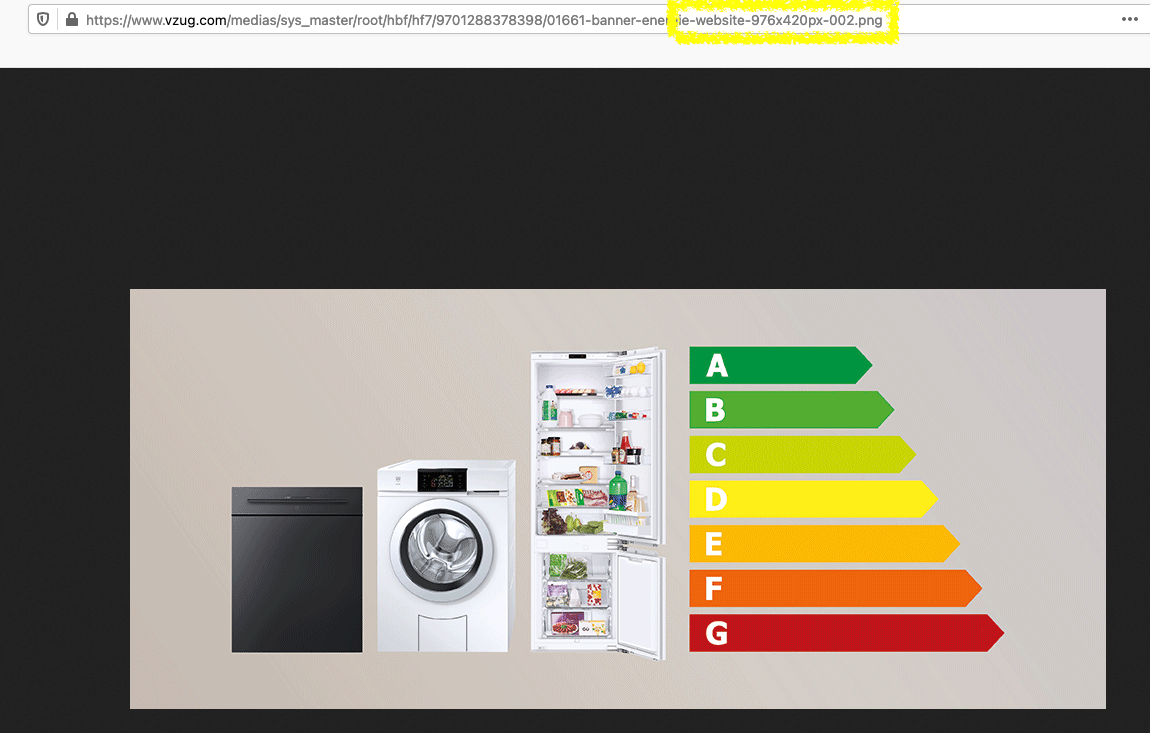
\includegraphics[scale=0.25]{vzug}
	\end{itemize}
		
	Lösung: Unser ImgProcessing CDN Service führt dies \textbf{on-the-fly} durch und bietet zugleich eine \textit{REST API}.
		
\end{frame}

\begin{frame}{Setup}{2. Technologien}
	\begin{itemize}
		\item{Backend}
		\begin{itemize}
			\item{\href{https://golang.org/}{go} (1.16.3)}
			\begin{itemize}
				\item{\href{https://gin-gonic.com/}{gin} (1.6.2)}
				\item{JWT}
			\end{itemize}
		\end{itemize}
		\item{Frontend}
		\begin{itemize}
			\item{\href{https://reactjs.org/versions/}{ReactJS} (17.0.2)}
			\begin{itemize}
				\item{Material-UI}
				\item{Ausgeliefert durch \href{https://nginx.org/}{Nginx} (1.19.9)}
			\end{itemize}
		\end{itemize}
		\item{Loadbalancer}
		       
		\begin{itemize}
			\item{\href{https://traefik.io/}{Traefik} (2.4.8)}
		\end{itemize} 
		\item{Storage}
		\begin{itemize}
			\item{\href{https://www.postgresql.org/}{PostgreSQL} (13.2)}
			\item{\href{https://min.io/}{MinIO - Object Storage} (RELEASE.2021-03-26)}
		\end{itemize}
		\item{Präsentation}
		\begin{itemize}
			\item{\href{https://github.com/ost-fh/Latex-Beamer-Theme}{LaTeX}}
		\end{itemize}       
	\end{itemize}
		
\end{frame}




\begin{frame}{Infrastruktur}{2. Technologien}
	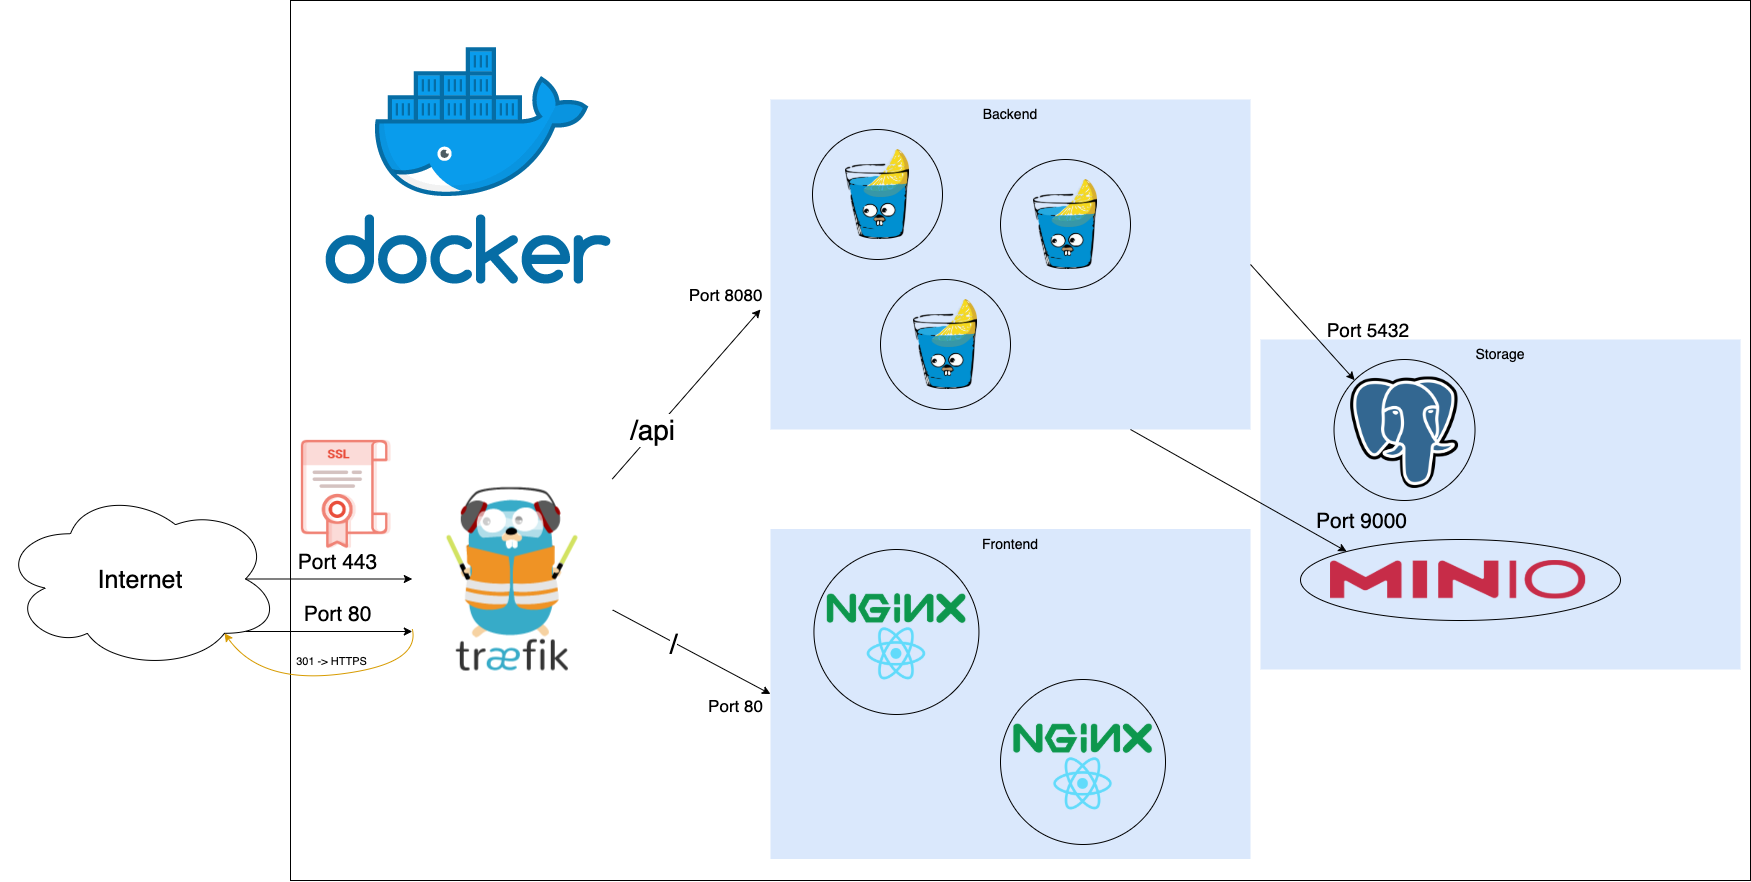
\includegraphics[scale=0.45]{Infrastruktur}	
\end{frame}

\begin{frame}{Datenmodell}{3. Entwicklung}
	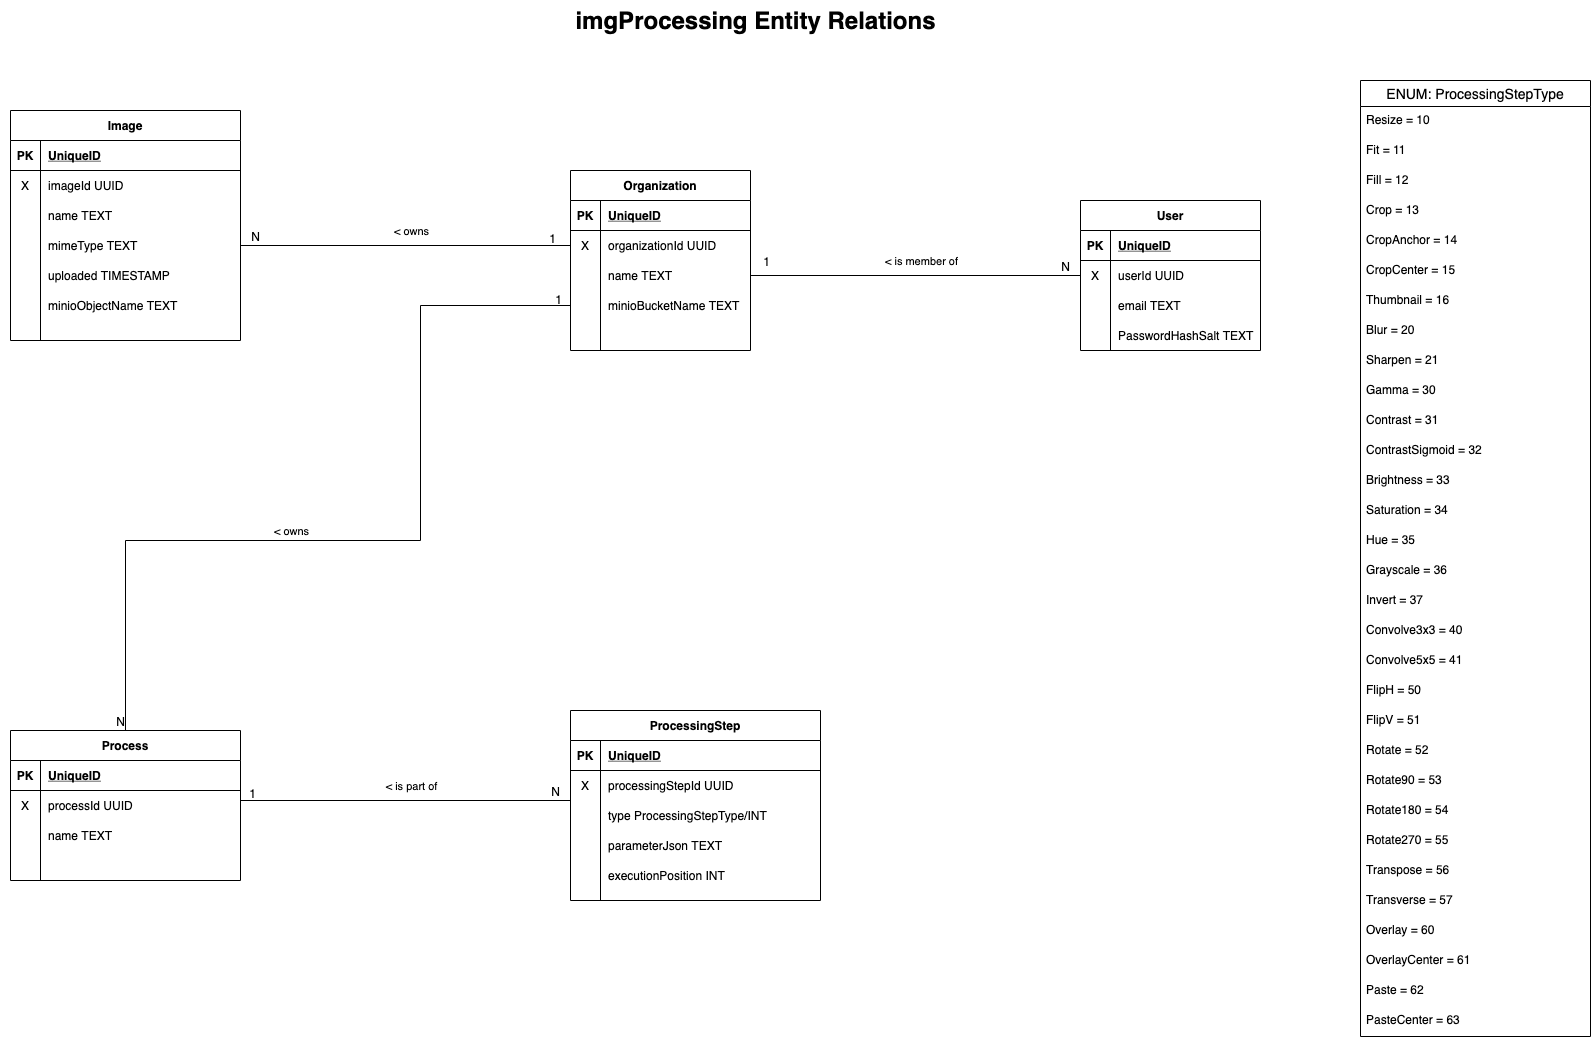
\includegraphics[scale=0.40]{db_model}	
\end{frame}

\begin{frame}{Github Actions}{3. Entwicklung}
	\begin{itemize}
		\item{Docker Images - builded and versioned by Github Actions}
		\begin{itemize}
			\item{Frontend}
			\item{Backend}
		\end{itemize}
		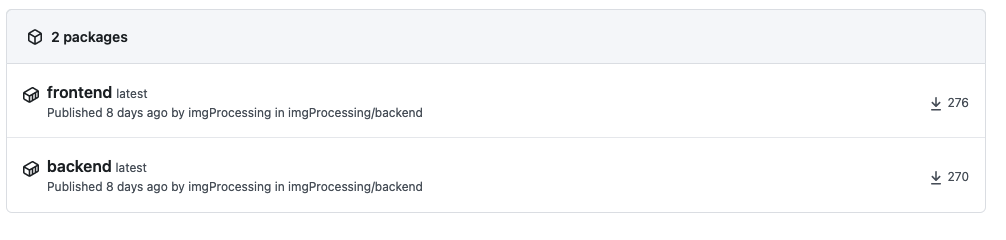
\includegraphics[scale=0.8]{action}
	\end{itemize}
\end{frame}

\begin{frame}{Demo}{}
	\href{https://imgprocessing.pesc.xyz/}{https://imgprocessing.pesc.xyz}
\end{frame}

\begin{frame}{End}{}
	\href{https://github.com/imgProcessing/backend}{Source Code}
\end{frame}

\end{document}